\documentclass{beamer}

% There are many different themes available for Beamer. A comprehensive
% list with examples is given here:
% http://deic.uab.es/~iblanes/beamer_gallery/index_by_theme.html
% You can uncomment the themes below if you would like to use a different
% one:
%\usetheme{AnnArbor}
%\usetheme{Antibes}
%\usetheme{Bergen}
%\usetheme{Berkeley}
%\usetheme{Berlin}
%\usetheme{Boadilla}
%\usetheme{boxes}
%\usetheme{CambridgeUS}
%\usetheme{Copenhagen}
%\usetheme{Darmstadt}
%\usetheme{default}
%\usetheme{Frankfurt}
%\usetheme{Goettingen}
%\usetheme{Hannover}
%\usetheme{Ilmenau}
%\usetheme{JuanLesPins}
%\usetheme{Luebeck}
%\usetheme{Madrid}
%\usetheme{Malmoe}
%\usetheme{Marburg}
%\usetheme{Montpellier}
%\usetheme{PaloAlto}
%\usetheme{Pittsburgh}
\usetheme{Rochester}
%\usetheme{Singapore}
%\usetheme{Szeged}
%\usetheme{Warsaw}

\usepackage[utf8x]{inputenc}
\usepackage[T1]{fontenc}
\usepackage[french]{babel}

\title{LSINF1225 : Programmation orientée-objet et gestion de données}

% A subtitle is optional and this may be deleted
\subtitle{UCLove}

\author{D.~Schmitz\inst{1} \and C.~Deknop\inst{2} \and R.~Gielen\inst{3} \and A.~Deronne\inst{4} \and M.~Volon\inst{5}}
% - Give the names in the same order as the appear in the paper.
% - Use the \inst{?} command only if the authors have different
%   affiliation.

\institute[Université de Louvain-la-Neuve] % (optional, but mostly needed)
{
  \inst{1}%
  SINF11BA
  \and
  \inst{2}%
  SINF12BA
  \and
  \inst{3}%
  SINF12BA
  \and
  \inst{4}%
  SINF12BA
  \and
  \inst{5}%
  LING2MS/LA
  }
% - Use the \inst command only if there are several affiliations.
% - Keep it simple, no one is interested in your street address.

\date{UCLove, 2016}
% - Either use conference name or its abbreviation.
% - Not really informative to the audience, more for people (including
%   yourself) who are reading the slides online

\subject{Theoretical Computer Science}
% This is only inserted into the PDF information catalog. Can be left
% out. 

% If you have a file called "university-logo-filename.xxx", where xxx
% is a graphic format that can be processed by latex or pdflatex,
% resp., then you can add a logo as follows:

% \pgfdeclareimage[height=0.5cm]{university-logo}{university-logo-filename}
% \logo{\pgfuseimage{university-logo}}

% Delete this, if you do not want the table of contents to pop up at
% the beginning of each subsection:
\AtBeginSubsection[]
{
  \begin{frame}<beamer>{Sommaire}
    \tableofcontents[currentsection,currentsubsection]
  \end{frame}
}

% Let's get started
\begin{document}

\begin{frame}
  \titlepage
\end{frame}

\begin{frame}{Sommaire}
  \tableofcontents
  % You might wish to add the option [pausesections]
\end{frame}

% Section and subsections will appear in the presentation overview
% and table of contents.
\section{Introduction}

\subsection{UCLove...?}
\begin{frame}{UCLove...?}
\begin{block}{Application de rencontres}
	\begin{itemize}
		\item{
			accessibilité (tablette/téléphone Android)
		}
		\item{
			efficacité, rapidité (public hétérogène ou recherche ciblée)
		}
		\item{
			éthique, confidentialité (visibilité des informations personnelles)
		}
	\end{itemize}
\end{block}
\begin{block}{Attentes "classiques"}
	\begin{itemize}
		\item{
			recherche de personnes (filtres disponibles)
		}
		\item{
			discussion instantanée
		}
		\item{
			[organisation d'une rencontre réelle]
		}
	\end{itemize}
\end{block}
\begin{block}{Présentation des fonctionnalités de base}
\end{block}
\end{frame}


\section{Aperçu de l'application}

\subsection*{Page d'accueil}

\begin{frame}{Page d'accueil}
  \begin{columns}
\begin{column}{0.4\textwidth}
\begin{itemize}[<+->]
\item Connexion
\end{itemize}
\end{column}
\begin{column}{0.6\textwidth}
\includegraphics<1>[width=2cm]{pictures/login.png}

\end{column}
\end{columns}
\end{frame}

\subsection*{Inscription}

\begin{frame}{Inscription}
  \begin{columns}
\begin{column}{0.4\textwidth}
\begin{itemize}[<+->]
\item Inscription
\end{itemize}
\end{column}
\begin{column}{0.6\textwidth}
\includegraphics<1>[width=2cm]{pictures/inscription.png}

\end{column}
\end{columns}
\end{frame}

\subsection*{Menu principal}


\begin{frame}{Menu Principal}
  \begin{columns}
\begin{column}{0.4\textwidth}
\begin{itemize}[<+->]
\item Navigation
\end{itemize}
\end{column}
\begin{column}{0.6\textwidth}
\includegraphics<1>[width=2cm]{pictures/Menu.png}

\end{column}
\end{columns}
\end{frame}

\subsection*{Profil}

\begin{frame}{Profil}
  \begin{columns}
\begin{column}{0.4\textwidth}
\begin{itemize}[<+->]
\item Nom
\item Attributs physiques
\item Photo
\end{itemize}
\end{column}
\begin{column}{0.6\textwidth}
\includegraphics<1>[width=2cm]{pictures/Profile.png}

\end{column}
\end{columns}
\end{frame}

\subsection*{Rencontre}
\begin{frame}{Rencontre}
  \begin{columns}
\begin{column}{0.4\textwidth}
\begin{itemize}[<+->]
\item Profil d'un utilisateur
\item Possibilité d'envoyer une requête ou de passer au profil suivant
\item Filtre disponible
\end{itemize}
\end{column}
\begin{column}{0.6\textwidth}
\includegraphics<1>[width=2cm]{pictures/Match.png}

\end{column}
\end{columns}
\end{frame}

\subsection*{Requêtes}
\begin{frame}{Requêtes}
  \begin{columns}
\begin{column}{0.4\textwidth}
\begin{itemize}[<+->]
\item Demandes en attente
\item Demande d'ajout d'autres utilisateurs
\end{itemize}
\end{column}
\begin{column}{0.6\textwidth}
\includegraphics<1>[width=2cm]{pictures/Requests.png}

\end{column}
\end{columns}
\end{frame}



\subsection*{Amis}
\begin{frame}{Amis}
  \begin{columns}
\begin{column}{0.4\textwidth}
\begin{itemize}[<+->]
\item Liste d'utilisateurs ajoutés
\item Utilisateur favoris
\end{itemize}
\end{column}
\begin{column}{0.6\textwidth}
\includegraphics<1>[width=2cm]{pictures/friends.png}

\end{column}
\end{columns}
\end{frame}

\subsection*{Options}
\begin{frame}{Options}
  \begin{columns}
\begin{column}{0.4\textwidth}
\begin{itemize}[<+->]
\item Choix de la langue
\item Déconnexion
\end{itemize}
\end{column}
\begin{column}{0.6\textwidth}
\includegraphics<1>[width=2cm]{pictures/Preferences.png}

\end{column}
\end{columns}
\end{frame}

\subsection*{Disponibilités}
\begin{frame}{Options}
  \begin{columns}
\begin{column}{0.4\textwidth}
\begin{itemize}[<+->]
\item un item
\end{itemize}
\end{column}
\begin{column}{0.6\textwidth}
\includegraphics<1>[width=2cm]{pictures/Disponibilities.png}

\end{column}
\end{columns}
\end{frame}


\section{Aspects techniques}

\subsection{Base de données}

\begin{frame}
  \begin{figure} 
  	\centering 
  	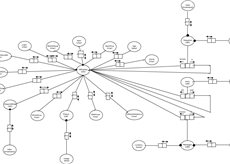
\includegraphics[scale=0.9]{pictures/schema_database.jpg} 
  	\caption{Schéma de la base de donnée} 
  	\label{fig:my_label} 
  \end{figure}
\end{frame}



\subsection{Implémentation}
<<<<<<< HEAD
\begin{frame}{Implémentation}
  \begin{itemize}
      \item{}
  \end{itemize}
=======
\begin{frame}
  \begin{figure} 
	\centering 
	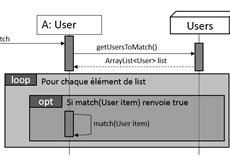
\includegraphics[scale=0.8]{pictures/sequence_match.jpg} 
	\caption{Diagramme de séquence pour l'activity Match} 
	\label{fig:my_label} 
  \end{figure}
>>>>>>> 568e5378bf7f6ee113bf792f9d6de0016127e413
\end{frame}

\section{Conclusion}

\subsection{Bilan}
\begin{frame}{Bilan}
\begin{block}{UCLove}
    \begin{itemize}
        \item{
            Prototype
        }
        \item{
            Priorité sur l'aspect fonctionnel de l'application
        }
    \end{itemize}
\end{block}
\end{frame}

\subsection{Perspectives}
\begin{frame}{Perspectives}
\begin{block}{Perspectives}
	\begin{itemize}
		\item{
			Disponibilités
		}
		\item{
			Confidentialité
		}
		\item{
			Interface graphique originale
		}
		\item{
			Base de données sur un serveur distant
		}
	\end{itemize}
\end{block}
\end{frame}

\end{document}


